% Two orthogonal adapter axes: interposer (WHERE) x interconnect (HOW DENSELY)
\documentclass[border=4pt]{standalone}
\usepackage{tikz}
\usetikzlibrary{arrows.meta, positioning, calc, fit, backgrounds,
                decorations.pathreplacing}
\usepackage[T1]{fontenc}
\usepackage{lmodern}

\definecolor{IHPfg}{RGB}{0,80,139}
\definecolor{IHPaccent}{RGB}{109,112,114}
\definecolor{IHPlight}{RGB}{225,238,250}
\definecolor{cDesigns}{RGB}{120,70,150}

\begin{document}
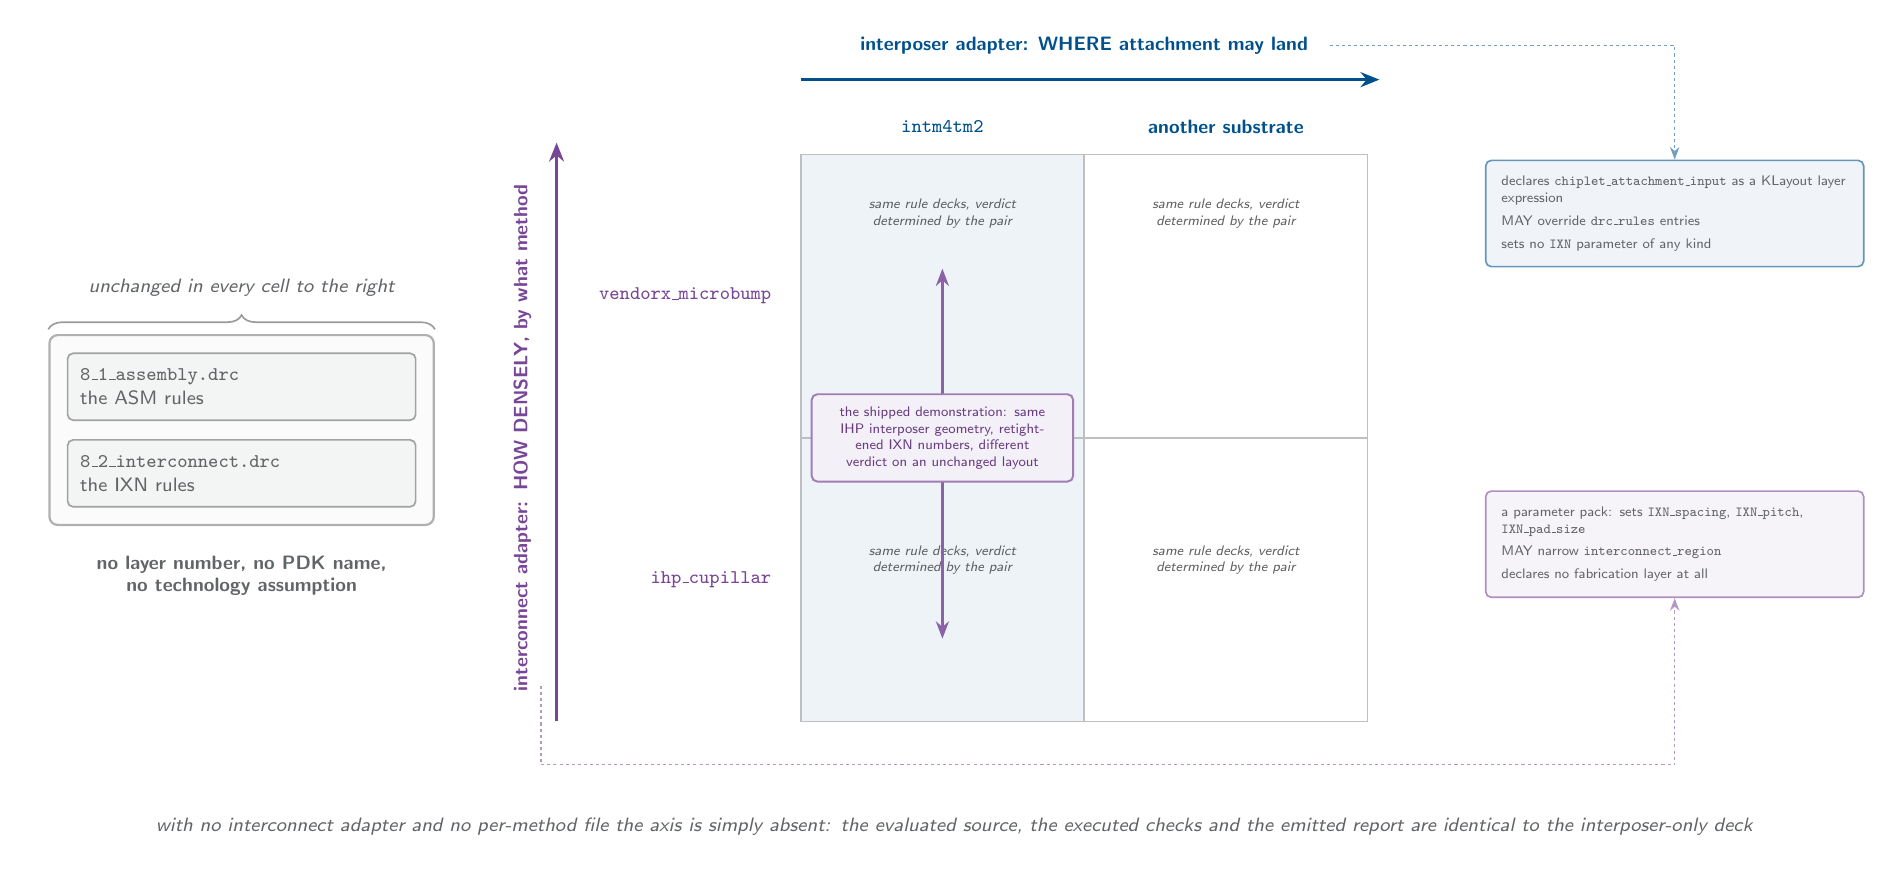
\begin{tikzpicture}[
    >=Stealth,
    % ---- the fixed core, at the far left ----
    adkslab/.style={
        rectangle, rounded corners=2pt,
        draw=IHPaccent!65, fill=IHPaccent!8, line width=0.6pt,
        text width=41mm, minimum height=8.5mm, inner sep=1.6mm,
        font=\sffamily\scriptsize, text=IHPaccent!90!black, align=left
    },
    adkcorebox/.style={
        rectangle, rounded corners=3pt,
        draw=IHPaccent!55, line width=0.8pt, fill=IHPaccent!3,
        inner xsep=2.2mm, inner ysep=2.2mm
    },
    adkcap/.style={
        font=\sffamily\scriptsize\bfseries, text=IHPaccent!90!black,
        text width=52mm, align=center
    },
    adkbrace/.style={
        decorate, decoration={brace, amplitude=1.8mm, raise=0.6mm},
        draw=IHPaccent!70, line width=0.6pt
    },
    adkbracelbl/.style={
        font=\sffamily\scriptsize\itshape, text=IHPaccent!90!black, align=center
    },
    % ---- the two by two grid ----
    adkcell/.style={draw=IHPaccent!45, line width=0.6pt},
    adkcelltxt/.style={
        font=\sffamily\tiny\itshape, text=IHPaccent!85!black,
        text width=29mm, align=center
    },
    adkcolhead/.style={
        font=\sffamily\scriptsize\bfseries, text=IHPfg, align=center
    },
    adkrowhead/.style={
        font=\sffamily\scriptsize\bfseries, text=cDesigns, align=right
    },
    % ---- axes ----
    adkaxisarr/.style={
        -{Stealth[length=2.4mm, width=1.9mm]}, line width=1.1pt, color=#1
    },
    adkaxislbl/.style={
        font=\sffamily\scriptsize\bfseries, text=#1, align=center
    },
    % ---- cards and leaders ----
    adkcard/.style={
        rectangle, rounded corners=2pt,
        draw=#1!60, fill=#1!6, line width=0.6pt,
        text width=44mm, inner sep=2mm,
        font=\sffamily\tiny, text=IHPaccent!90!black, align=left
    },
    adklead/.style={
        -{Stealth[length=1.6mm]}, line width=0.5pt, color=#1!55, dash pattern=on 1.1pt off 1.1pt
    },
    adkswap/.style={
        {Stealth[length=2.2mm]}-{Stealth[length=2.2mm]}, line width=1pt, color=cDesigns!85
    },
    adkcallout/.style={
        rectangle, rounded corners=2pt,
        draw=cDesigns!70, fill=cDesigns!8, line width=0.7pt,
        text width=30mm, inner sep=1.6mm,
        font=\sffamily\tiny, text=cDesigns!85!black, align=center
    },
    adkfoot/.style={
        font=\sffamily\scriptsize\itshape, text=IHPaccent!90!black,
        text width=205mm, align=center
    }
]

% =====================================================================
% CORE: the rule decks that never change
% =====================================================================
\node[adkslab] (asm) at (-0.1, -1.15)
    {\textbf{\ttfamily 8\_1\_assembly.drc}\\[0.3mm]the ASM rules};
\node[adkslab] (ixn) at (-0.1, -2.25)
    {\textbf{\ttfamily 8\_2\_interconnect.drc}\\[0.3mm]the IXN rules};

\begin{pgfonlayer}{background}
  \node[adkcorebox, fit=(asm)(ixn)] (core) {};
\end{pgfonlayer}

\draw[adkbrace] (core.north west) -- (core.north east);
\node[adkbracelbl, anchor=south, text width=52mm]
    at ([yshift=3.6mm]core.north) {unchanged in every cell to the right};

\node[adkcap, anchor=north] at ([yshift=-2.6mm]core.south)
    {no layer number, no PDK name,\\no technology assumption};

% =====================================================================
% GRID: two by two
% =====================================================================
% highlighted column (intm4tm2)
\fill[IHPfg!7] (7.0,-5.4) rectangle (10.6,1.8);

\draw[adkcell] (7.0,-1.8)  rectangle (10.6, 1.8);
\draw[adkcell] (10.6,-1.8) rectangle (14.2, 1.8);
\draw[adkcell] (7.0,-5.4)  rectangle (10.6,-1.8);
\draw[adkcell] (10.6,-5.4) rectangle (14.2,-1.8);

\node[adkcelltxt] at (8.8,  1.05) {same rule decks, verdict determined by the pair};
\node[adkcelltxt] at (12.4, 1.05) {same rule decks, verdict determined by the pair};
\node[adkcelltxt] at (8.8, -3.35) {same rule decks, verdict determined by the pair};
\node[adkcelltxt] at (12.4,-3.35) {same rule decks, verdict determined by the pair};

% =====================================================================
% HORIZONTAL AXIS: the interposer adapter
% =====================================================================
\draw[adkaxisarr=IHPfg] (7.0, 2.75) -- (14.35, 2.75);
\node[adkaxislbl=IHPfg, anchor=south] (hlbl)
    at (10.6, 2.95) {interposer adapter: WHERE attachment may land};

\node[adkcolhead] at (8.8,  2.15) {\ttfamily intm4tm2};
\node[adkcolhead] at (12.4, 2.15) {another substrate};

% =====================================================================
% VERTICAL AXIS: the interconnect adapter
% =====================================================================
\draw[adkaxisarr=cDesigns] (3.9, -5.4) -- (3.9, 1.95);
\node[adkaxislbl=cDesigns, rotate=90, anchor=south, text width=72mm] (vlbl)
    at (3.7, -1.8) {interconnect adapter: HOW DENSELY, by what method};

\node[adkrowhead, anchor=east] at (6.75,  0.0) {\ttfamily vendorx\_microbump};
\node[adkrowhead, anchor=east] at (6.75, -3.6) {\ttfamily ihp\_cupillar};

% =====================================================================
% THE SHIPPED DEMONSTRATION: vertical swap inside the intm4tm2 column
% =====================================================================
\draw[adkswap] (8.8, 0.35) -- (8.8, -4.35);
\node[adkcallout] at (8.8, -1.8)
    {the shipped demonstration: same IHP interposer geometry, retightened IXN
     numbers, different verdict on an unchanged layout};

% =====================================================================
% WHAT EACH AXIS SUPPLIES
% =====================================================================
\node[adkcard=IHPfg] (carda) at (18.1, 1.05)
    {declares {\ttfamily chiplet\_attachment\_input} as a KLayout layer
     expression\\[0.8mm]
     MAY override {\ttfamily drc\_rules} entries\\[0.8mm]
     sets no {\ttfamily IXN} parameter of any kind};

\node[adkcard=cDesigns] (cardb) at (18.1, -3.15)
    {a parameter pack: sets {\ttfamily IXN\_spacing}, {\ttfamily IXN\_pitch},
     {\ttfamily IXN\_pad\_size}\\[0.8mm]
     MAY narrow {\ttfamily interconnect\_region}\\[0.8mm]
     declares no fabrication layer at all};

\draw[adklead=IHPfg] ([xshift=1.5mm]hlbl.east) -| (carda.north);

\draw[adklead=cDesigns] (3.7,-4.95) -- (3.7,-5.95) -| (cardb.south);

% =====================================================================
% FOOTER
% =====================================================================
\node[adkfoot, anchor=north] at (8.95, -6.5)
    {with no interconnect adapter and no per-method file the axis is simply
     absent: the evaluated source, the executed checks and the emitted report
     are identical to the interposer-only deck};

\end{tikzpicture}
\end{document}
